\chapter{Cytoskeleton Dynamics and Cell Motility}\label{ch:b3:cytoskeleton-motility}

A neutrophil chasing a bacterium through a tissue crawls at ten
micrometres a minute, changing direction within seconds when the scent
shifts. A vesicle of neurotransmitter made in the cell body of a motor
neuron travels a metre down the axon to the foot, hauled by a motor
protein that takes eight-nanometre steps, a hundred a second, for a
fortnight. The cilia lining the windpipe beat twelve times a second in
coordinated waves that carry a day's inhaled dust up to the throat. All
of this is done by three kinds of protein filament that assemble and
disassemble in seconds, and by motors that burn one molecule of ATP per
step. The cytoskeleton is not a skeleton at all in the sense of a fixed
frame; it is a set of polymers in constant turnover, whose dynamics
\emph{are} the mechanism of shape, division and movement. This chapter
treats the polymers and their kinetics, the motors and the physics that
limits them, the crawling of a cell, and the beating of cilia and
flagella.

\section{Three polymers}

\begin{definition}[Actin filaments, microtubules, intermediate filaments]\label{def:b3:cytoskeleton-motility:filaments}
\index{actin filament}\index{microtubule}\index{intermediate filament}\index{polarity!of filaments}\index{centrosome}
An \emph{actin filament} is a two-stranded helical polymer of globular
actin, \qty{7}{nm} thick, each subunit \qty{2.7}{nm} along the axis,
polar: the \emph{barbed} (plus) end grows faster than the \emph{pointed}
(minus) end, and each subunit carries an ATP that is hydrolysed after
incorporation. A \emph{microtubule} is a hollow tube of \qty{25}{nm}
outer diameter built from thirteen protofilaments of $\alpha\beta$-tubulin
dimers (\qty{8}{nm} per dimer), also polar, its \emph{plus} end growing
faster and its \emph{minus} end usually anchored at the
\emph{centrosome} near the nucleus; the $\beta$ subunit hydrolyses its
GTP after incorporation. An \emph{intermediate filament} is a rope of
\qty{10}{nm} made of coiled-coil proteins (keratins in epithelia,
vimentin in mesenchyme, neurofilaments in axons, lamins under the
nuclear envelope), apolar, without nucleotide, and far more stable ---
a tension-bearing cable rather than a dynamic track. Actin sits mostly
under the plasma membrane and in protrusions; microtubules radiate from
the centrosome and serve as the tracks of long-range transport and as
the spindle; intermediate filaments give a cell and its nucleus their
mechanical resilience.
\end{definition}

\begin{omfigure}
\begin{tikzpicture}[every node/.style={font=\scriptsize}, >=stealth]
  % actin
  \begin{scope}
    \foreach \i in {0,...,11} { \fill[omThm!70] ({\i*0.4},{0.12*sin(\i*60)}) circle (0.17); }
    \node[below, align=center] at (2.2,-0.5) {actin filament, \qty{7}{nm}\\two-stranded helix, ATP-actin\\subunit \qty{2.7}{nm} along the axis};
    \node[left] at (-0.3,0) {$-$ pointed}; \node[right] at (4.6,0) {barbed $+$};
  \end{scope}
  % microtubule
  \begin{scope}[xshift=7.2cm]
    \draw[thick, fill=omDef!25] (0,-0.55) rectangle (4.4,0.55);
    \foreach \y in {-0.35,-0.15,0.05,0.25} \draw[omDef] (0,\y) -- (4.4,\y);
    \foreach \x in {0.4,0.8,...,4.0} \draw[omDef] (\x,-0.55) -- (\x,0.55);
    \draw[thick] (4.4,0) ellipse (0.18 and 0.55); \draw[thick, fill=white] (4.4,0) ellipse (0.09 and 0.38);
    \node[below, align=center] at (2.2,-0.65) {microtubule, \qty{25}{nm}\\13 protofilaments of $\alpha\beta$-tubulin (GTP)\\dimer \qty{8}{nm} long};
    \node[left] at (-0.2,0) {$-$}; \node[right] at (4.7,0) {$+$};
  \end{scope}
  % intermediate filament
  \begin{scope}[yshift=-2.9cm, xshift=3.6cm]
    \foreach \dd in {-0.12,0,0.12} \draw[omMeth!70!black, thick] plot[domain=0:4.4, samples=60] (\x, {\dd + 0.1*sin(\x*200 + \dd*400)});
    \node[below, align=center] at (2.2,-0.4) {intermediate filament, \qty{10}{nm}\\coiled-coil rope (keratin, vimentin, lamin), no polarity, no nucleotide};
  \end{scope}
\end{tikzpicture}

{\small The three filaments to scale in diameter. Actin and tubulin
polymers are polar and hydrolyse a nucleotide after assembly, which is
what makes them dynamic; the \omterm{def:b3:cytoskeleton-motility:filaments}{intermediate filament} is an apolar rope
built for endurance.}
\end{omfigure}

\begin{omfigure}
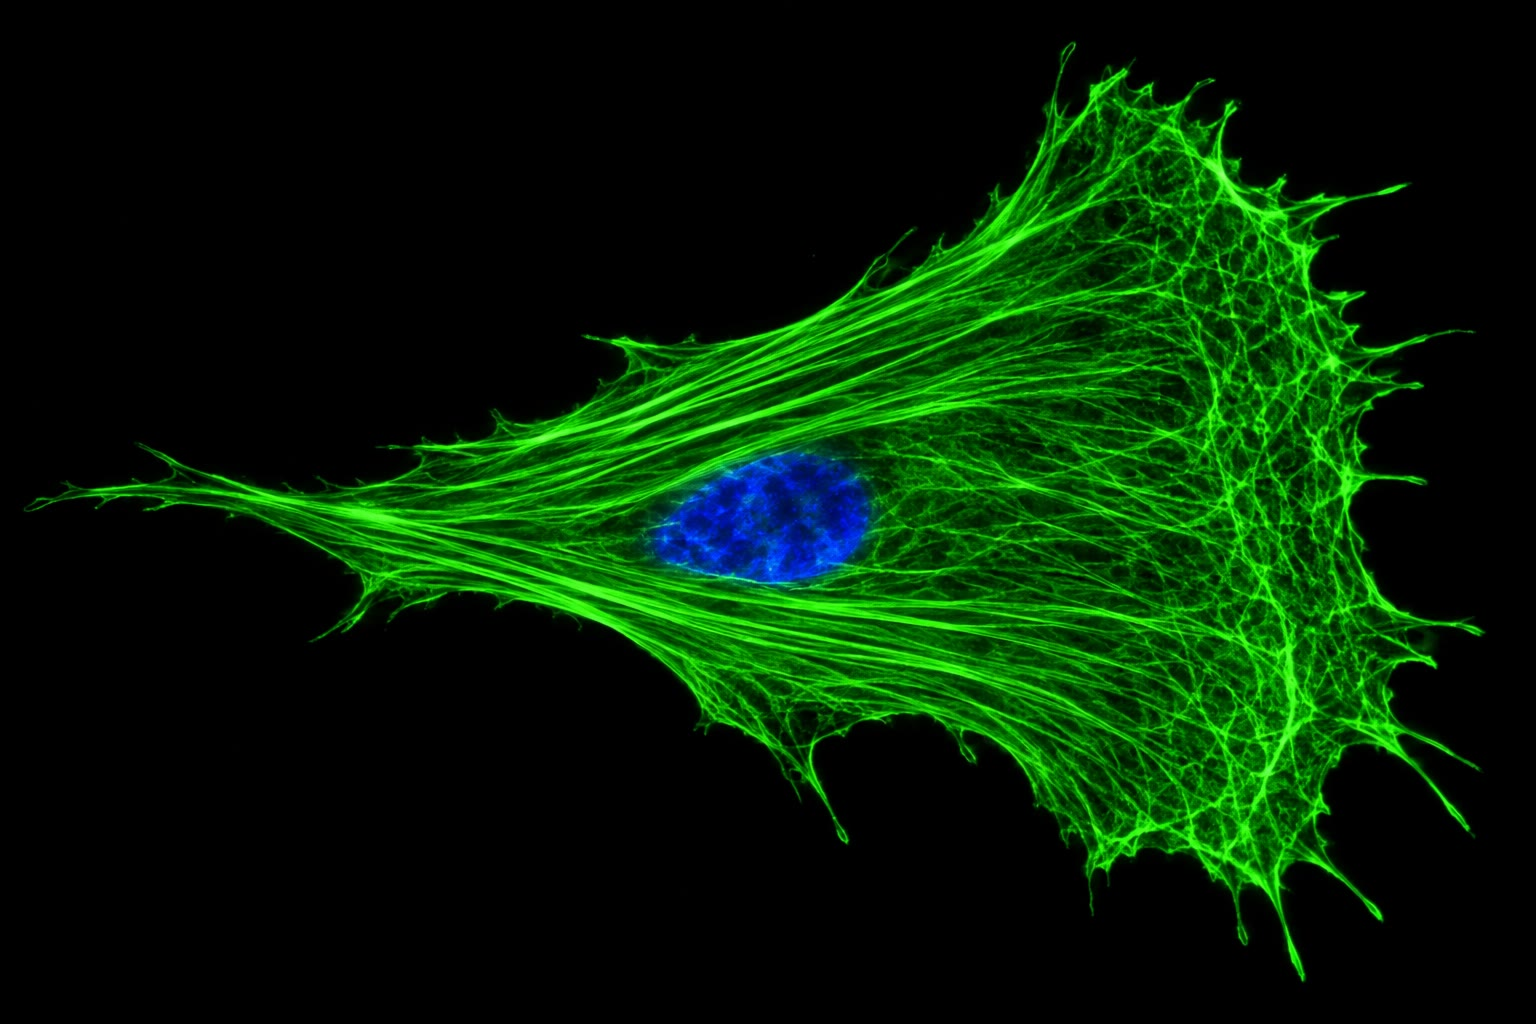
\includegraphics[width=0.54\linewidth]{images/book5/ai/b5-09-fibroblast-actin.jpg}\hspace{0.03\linewidth}
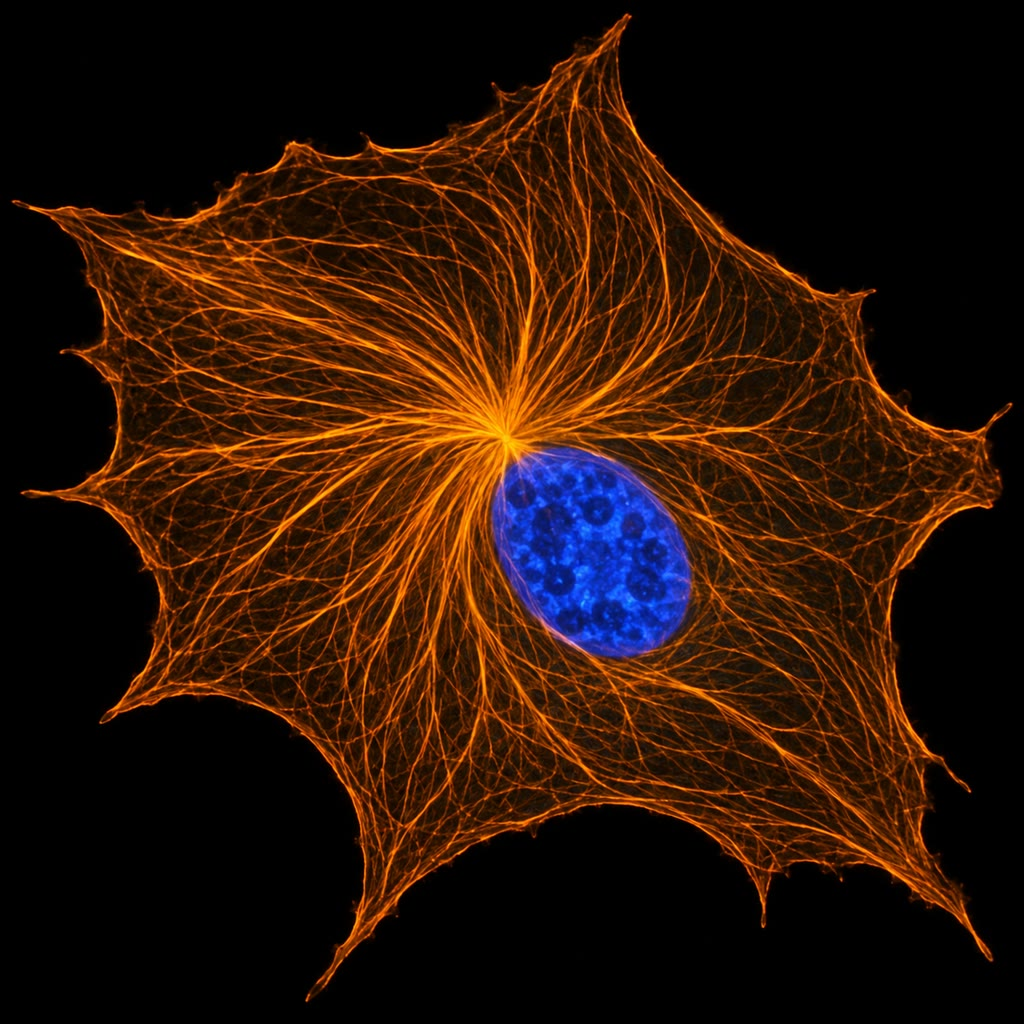
\includegraphics[width=0.36\linewidth]{images/book5/ai/b5-09-microtubules.jpg}

{\small Left: actin (green) in a migrating fibroblast --- stress fibres
across the body, a dense meshwork at the broad leading edge on the
right. Right: \omterm{def:b3:cytoskeleton-motility:filaments}{microtubules} (orange) radiating from the \omterm{def:b3:cytoskeleton-motility:filaments}{centrosome}
beside the nucleus (blue) to the cell margin.}
\end{omfigure}

\section{The kinetics of a polymer}

\begin{theorem}[Critical concentration and treadmilling]\label{thm:b3:cytoskeleton-motility:treadmilling}
\index{critical concentration}\index{treadmilling}
Let an end of a filament add subunits at rate $k_{\text{on}}C$, with
$C$ the free monomer concentration, and lose them at rate
$k_{\text{off}}$. The end grows if $C$ exceeds its \emph{\omterm{thm:b3:cytoskeleton-motility:treadmilling}{critical
concentration}} $C_{c} = k_{\text{off}}/k_{\text{on}}$ and shrinks below
it. If the two ends have different \omterm{thm:b3:cytoskeleton-motility:treadmilling}{critical concentrations}, $C_{c}^{+}
< C_{c}^{-}$, then at the steady state where the filament neither
lengthens nor shortens the monomer concentration is
\[
C_{\text{ss}} = \frac{k_{\text{off}}^{+} + k_{\text{off}}^{-}}
{k_{\text{on}}^{+} + k_{\text{on}}^{-}},
\qquad C_{c}^{+} < C_{\text{ss}} < C_{c}^{-},
\]
and the plus end grows while the minus end shrinks at the same rate
$J = k_{\text{on}}^{+}C_{\text{ss}} - k_{\text{off}}^{+} > 0$: subunits
flow through the filament from plus to minus --- \emph{treadmilling}
--- at the cost of one nucleotide hydrolysed per subunit.
\end{theorem}
\begin{proof}
The net rate at an end is $k_{\text{on}}C - k_{\text{off}}$, zero at
$C_{c}$. Constant length requires the sum of the two net rates to
vanish, which gives $C_{\text{ss}}$; it lies between the two \omterm{thm:b3:cytoskeleton-motility:treadmilling}{critical
concentrations} because it is a weighted mean of them ($C_{\text{ss}} =
(k_{\text{on}}^{+}C_{c}^{+} + k_{\text{on}}^{-}C_{c}^{-})/(k_{\text{on}}^{+}
+ k_{\text{on}}^{-})$). Above $C_{c}^{+}$ the plus end grows; below
$C_{c}^{-}$ the minus end shrinks; the flux is the plus end's net rate.
Two ends of the same chemical polymer would have the same $C_{c}$ (the
same equilibrium constant), so a difference requires that the subunit
change after incorporation --- the hydrolysis of ATP or GTP --- which
makes the ends differ and pays for the flow.
\end{proof}

\begin{example}[Actin in the test tube]\label{ex:b3:cytoskeleton-motility:actin-numbers}
For actin-ATP, $k_{\text{on}}^{+} = \qty{11.6}{\micro M^{-1}.s^{-1}}$,
$k_{\text{off}}^{+} = \qty{1.4}{s^{-1}}$ ($C_{c}^{+} = \qty{0.12}{\micro
M}$); $k_{\text{on}}^{-} = \qty{1.3}{\micro M^{-1}.s^{-1}}$,
$k_{\text{off}}^{-} = \qty{0.8}{s^{-1}}$ ($C_{c}^{-} = \qty{0.6}{\micro
M}$). Then $C_{\text{ss}} = 2.2/12.9 = \qty{0.17}{\micro M}$ and $J =
11.6\times 0.17 - 1.4 = 0.6$ subunits per second: \qty{1.6}{nm/s},
imperceptible. In a cell the filaments treadmill a hundred times
faster, because cofilin severs and strips the old ADP-actin from the
pointed ends, profilin loads fresh ATP-actin onto barbed ends, and
capping proteins decide which barbed ends may grow at all: the bare
polymer supplies the mechanism, the regulators supply the speed.
\end{example}

\begin{omfigure}
\begin{tikzpicture}
\begin{axis}[
  width=0.7\linewidth, height=5.6cm,
  axis x line=bottom, axis y line=left,
  xmin=0, xmax=1.0, ymin=-1.6, ymax=4,
  xlabel={free actin ($\unit{\micro M}$)}, ylabel={net rate (subunits/s)},
  xlabel style={font=\small, at={(axis description cs:0.5,-0.12)}, anchor=north},
  ylabel style={font=\small},
  tick label style={font=\small}, xtick={0,0.2,0.4,0.6,0.8,1.0}, ytick={-1,0,1,2,3,4},
  clip=false,
]
\addplot[thin, gray, domain=0:1.0, samples=2] {0};
\addplot[very thick, omThm, domain=0:0.46, samples=2] {11.6*x-1.4};
\addplot[very thick, omDef, domain=0:1.0, samples=2] {1.3*x-0.8};
\draw[dashed, gray] (axis cs:0.17,-1.6) -- (axis cs:0.17,4);
\node[font=\scriptsize, omThm, anchor=south east] at (axis cs:0.44,3.1) {barbed end};
\node[font=\scriptsize, omDef, anchor=north west] at (axis cs:0.62,-0.25) {pointed end};
\node[font=\scriptsize, anchor=south west] at (axis cs:0.19,3.5) {$C_{\text{ss}}$};
\fill[omThm] (axis cs:0.12,0) circle (2pt); \node[font=\scriptsize, anchor=north east] at (axis cs:0.11,-0.05) {$C_{c}^{+}$};
\fill[omDef] (axis cs:0.6,0) circle (2pt); \node[font=\scriptsize, anchor=south west] at (axis cs:0.61,0.05) {$C_{c}^{-}$};
\end{axis}
\end{tikzpicture}

{\small Net growth rate of each end of an \omterm{def:b3:cytoskeleton-motility:filaments}{actin filament} against free
monomer, with the rate constants of the example. Between the two
\omterm{thm:b3:cytoskeleton-motility:treadmilling}{critical concentrations} the barbed end grows and the pointed end
shrinks; at the dashed line the two exactly cancel and the filament
treadmills.}
\end{omfigure}

\begin{definition}[Dynamic instability]\label{def:b3:cytoskeleton-motility:instability}
\index{dynamic instability}\index{GTP cap}\index{catastrophe}
\omterm{def:b3:cytoskeleton-motility:filaments}{Microtubules} do something stranger than treadmilling. A growing plus
end carries a \emph{GTP cap} of freshly added dimers; behind it the GTP
is hydrolysed, and GDP-tubulin, which prefers a curved conformation,
is held straight in the lattice under strain. If the cap is lost --- the
end pauses, or growth slows --- the strained protofilaments peel
outward and the \omterm{def:b3:cytoskeleton-motility:filaments}{microtubule} shortens at \qty{300}{nm/s}, twenty times
its growth rate: a \emph{catastrophe}, which ends when a GTP dimer
lands and a new cap forms (a \emph{rescue}). In one population,
therefore, some \omterm{def:b3:cytoskeleton-motility:filaments}{microtubules} grow while neighbours collapse: this is
\emph{dynamic instability}. It lets a cell explore its own volume with
plus ends every few minutes and rebuild the whole array when the
\omterm{def:b3:cytoskeleton-motility:filaments}{centrosome} moves or the cell divides. The cell tunes it through
proteins that track plus ends, stabilise (tau, MAP2), sever (katanin)
or depolymerise (kinesin-13) \omterm{def:b3:cytoskeleton-motility:filaments}{microtubules}; the drugs colchicine and
the vinca alkaloids block assembly and taxol blocks disassembly, all
of them poisons of the mitotic spindle used against cancer.
\end{definition}

\begin{proof}[Evidence]
Mitchison and Kirschner (1984) watched populations of \omterm{def:b3:cytoskeleton-motility:filaments}{microtubules}
grown from \omterm{def:b3:cytoskeleton-motility:filaments}{centrosomes} in vitro. Diluting the tubulin below the
\omterm{thm:b3:cytoskeleton-motility:treadmilling}{critical concentration}, they expected all the \omterm{def:b3:cytoskeleton-motility:filaments}{microtubules} to shorten
slowly; instead the number of \omterm{def:b3:cytoskeleton-motility:filaments}{microtubules} fell while the survivors
kept growing --- some had disassembled completely and fast, others not
at all. Individual \omterm{def:b3:cytoskeleton-motility:filaments}{microtubules} filmed later by video microscopy
switched abruptly between phases of steady growth and rapid shrinkage.
The \omterm{def:b3:cytoskeleton-motility:instability}{GTP cap} explained both: only the capped ends grow, and the loss of
the cap is a rare, all-or-nothing event.
\end{proof}

\section{Motors}

\begin{definition}[Motor proteins]\label{def:b3:cytoskeleton-motility:motors}
\index{myosin}\index{kinesin}\index{dynein}\index{processivity}
A \emph{motor protein} converts the free energy of ATP hydrolysis into
directed movement along a filament: \emph{myosins} along actin (myosin
II, the muscle and contractile motor, toward the barbed end; myosin V,
a two-headed vesicle carrier stepping \qty{36}{nm}), \emph{kinesins}
along \omterm{def:b3:cytoskeleton-motility:filaments}{microtubules} toward the plus end (kinesin-1 steps \qty{8}{nm},
one tubulin dimer, per ATP, hand over hand, at about \qty{800}{nm/s}),
and \emph{dyneins} toward the minus end (cytoplasmic dynein, with its
adaptor dynactin, hauls cargo back to the cell centre; \omterm{def:b3:cytoskeleton-motility:cilia}{axonemal dyneins}
bend cilia). A motor is \emph{processive} if it takes many steps before
detaching: kinesin-1 walks about a micrometre, a hundred steps, alone;
a single myosin II head takes one stroke and lets go, so muscle needs
hundreds of heads working on one filament. Motors read the polarity of
the track, so a cell's geography --- plus ends at the periphery, minus
ends at the centre --- is a map of where each motor will take its
cargo.
\end{definition}

\begin{proof}[Evidence]
Vale, Reese and Sheetz (1985) found \omterm{def:b3:cytoskeleton-motility:motors}{kinesin} as the protein of squid
axoplasm that made latex beads glide along \omterm{def:b3:cytoskeleton-motility:filaments}{microtubules} in the plus
direction, and in the following years the two-headed structure, the
direction of each family and the retrograde partner \omterm{def:b3:cytoskeleton-motility:motors}{dynein} were sorted
out. Svoboda, Schmidt, Schnapp and Block (1993) held a bead carrying a
single \omterm{def:b3:cytoskeleton-motility:motors}{kinesin} in an optical trap and recorded its position with
nanometre resolution: the bead advanced in discrete steps of
\qty{8}{nm}, one per ATP at low ATP concentration, and stalled against
a force of about \qty{6}{pN}. The molecular staircase was seen
directly.
\end{proof}

\begin{omfigure}
\begin{tikzpicture}[every node/.style={font=\scriptsize}, >=stealth]
  % left: kinesin on a microtubule
  \begin{scope}
    \draw[thick, fill=omDef!25] (0,0) rectangle (5.4,0.5);
    \foreach \x in {0.4,0.8,...,5.2} \draw[omDef] (\x,0) -- (\x,0.5);
    \node[left] at (-0.1,0.25) {$-$}; \node[right] at (5.5,0.25) {$+$};
    % two heads, stalk, cargo
    \fill[omProp] (2.4,0.72) circle (0.2); \fill[omProp!60] (3.2,0.72) circle (0.2);
    \draw[thick, omProp!80!black] (2.6,0.85) -- (2.85,1.4) -- (3.05,0.85); \draw[thick, omProp!80!black] (2.85,1.4) -- (2.85,2.3);
    \draw[thick, fill=omExo!40] (2.85,2.7) circle (0.4); \node at (2.85,2.7) {cargo};
    \draw[->, thick, omThm] (3.4,0.72) arc[start angle=180, end angle=0, radius=0.4] ; \node[right, omThm] at (3.85,1.15) {\qty{8}{nm} per ATP};
    \node[below, align=center] at (2.7,-0.1) {kinesin-1 walks hand over hand toward the plus end;\\about $100$ steps a second, \qty{0.8}{\micro m/s}};
  \end{scope}
  % right: optical trap staircase
  \begin{scope}[xshift=7.2cm, yshift=-0.6cm]
  \begin{axis}[
    width=5.6cm, height=4.4cm, axis lines=left,
    xmin=0, xmax=1.0, ymin=0, ymax=40,
    xlabel={time (s)}, ylabel={position (nm)},
    xlabel style={font=\scriptsize, at={(axis description cs:0.5,-0.12)}, anchor=north},
    ylabel style={font=\scriptsize},
    tick label style={font=\scriptsize}, xtick={0,0.5,1.0}, ytick={0,8,16,24,32},
  ]
  \addplot[very thick, omProp!80!black, const plot] coordinates {(0,0) (0.18,8) (0.31,16) (0.55,24) (0.71,32) (1.0,32)};
  \end{axis}
  \node[font=\scriptsize, align=center] at (2.8,3.6) {a single motor in an optical trap,\\low ATP: \qty{8}{nm} steps};
  \end{scope}
\end{tikzpicture}

{\small \omterm{def:b3:cytoskeleton-motility:motors}{Kinesin} on its track and its footprint in an optical trap. The
two heads alternate, each step advancing the motor by one tubulin dimer,
\qty{8}{nm}; at low ATP the steps are separated by waits for the next
nucleotide and the staircase is seen directly.}
\end{omfigure}

\begin{proposition}[What physics allows a motor]\label{prop:b3:cytoskeleton-motility:physics}
\index{stall force}\index{thermal energy}\index{diffusion versus transport}
The hydrolysis of one ATP in the cell releases about \qty{50}{kJ/mol},
that is $8\times 10^{-20}$ J per molecule. A motor that advances $d$
per ATP against a force $F$ does work $Fd$, so its \emph{\omterm{prop:b3:cytoskeleton-motility:physics}{stall force}}
cannot exceed $F_{\max} = \Delta G/d$: for \omterm{def:b3:cytoskeleton-motility:motors}{kinesin}'s \qty{8}{nm} step,
\qty{10}{pN}; the measured \qty{6}{pN} means an efficiency near
\qty{60}{\%}, higher than any engine. The \omterm{prop:b3:cytoskeleton-motility:physics}{thermal energy} $k_{B}T =
4.1\times 10^{-21}$ J, or \qty{4.1}{pN.nm}, is only a twentieth of the
ATP energy but is delivered to the motor constantly as Brownian
kicks; a motor is a device that rectifies them, letting the head
diffuse forward and binding when it lands, so that the chemical energy
is spent on making the step irreversible rather than on pushing.
Transport by motor beats diffusion over any distance that matters in
a large cell: a vesicle with diffusion coefficient $D = \qty{1}{\micro
m^2/s}$ needs a time $L^{2}/2D$ to wander a distance $L$ --- half a
second for a micrometre, but \num{16000} years for a metre of axon ---
whereas a motor at \qty{1}{\micro m/s} covers the metre in twelve days.
\end{proposition}
\admitted

\section{How a cell crawls}

\begin{definition}[Cell migration]\label{def:b3:cytoskeleton-motility:migration}
\index{lamellipodium}\index{Arp2/3 complex}\index{focal adhesion}\index{integrin}\index{Rho GTPases}
A crawling cell repeats a cycle of four steps. \emph{Protrusion}: at
the leading edge actin polymerises against the membrane in a sheet, the
\emph{lamellipodium}, whose branched network is built by the
\emph{Arp2/3 complex}, which nucleates a new filament from the side of
an existing one at \qty{70}{\degree}, while capping protein limits each
filament's growth and cofilin recycles the network a few micrometres
back; finger-like \emph{filopodia} of bundled filaments probe ahead.
\emph{Adhesion}: the new protrusion attaches to the substrate through
\emph{integrins}, transmembrane receptors that bind matrix proteins
outside and, through adaptor proteins, actin inside, clustered in
\emph{focal adhesions}. \emph{Contraction}: \omterm{def:b3:cytoskeleton-motility:motors}{myosin} II pulls on the
stress fibres anchored at the adhesions, dragging the cell body
forward. \emph{Retraction}: the adhesions at the rear release and the
tail is pulled in. The cycle is coordinated by three \omterm{def:b3:membrane-traffic:coats}{small GTPases} of
the \emph{Rho} family --- Rac drives lamellipodia, Cdc42 filopodia,
Rho stress fibres and contraction --- which are the targets of the
receptors that read the direction of a chemical gradient
(chemotaxis) or the stiffness and pattern of the substrate.
\end{definition}

\begin{omfigure}
\begin{tikzpicture}[every node/.style={font=\scriptsize}, >=stealth]
  % substrate
  \draw[very thick, gray] (0,0) -- (12,0); \node[below right, gray] at (0,-0.05) {substrate (matrix)};
  % cell outline
  \draw[thick, omDef, fill=omDef!10] (1.0,0.05) .. controls (1.2,1.4) and (3.0,2.3) .. (5.0,2.2) .. controls (7.0,2.1) and (8.6,1.4) .. (9.8,0.6) .. controls (10.3,0.4) and (10.8,0.2) .. (11.2,0.05) -- cycle;
  % nucleus
  \draw[thick, fill=omDef!40] (4.6,1.1) ellipse (1.0 and 0.6); \node at (4.6,1.1) {nucleus};
  % lamellipodium: branched actin
  \foreach \p/\a in {(9.9,0.3)/20,(10.1,0.5)/-10,(10.3,0.25)/35,(10.6,0.45)/5,(10.4,0.7)/-25,(9.7,0.7)/15} { \draw[omThm, thick] \p -- ++(\a:0.55); \draw[omThm, thick] \p ++(\a:0.3) -- ++(\a+70:0.35); }
  \node[right, align=left, omThm] at (11.3,1.3) {1. protrusion:\\Arp2/3-branched actin\\pushes the membrane};
  \draw[->, thick, omThm] (11.3,0.3) -- (11.9,0.3);
  % focal adhesions
  \foreach \x in {9.3,7.6,2.4} \fill[omProp] (\x-0.25,0.03) rectangle (\x+0.25,0.18);
  \node[below, omProp, align=center] at (9.3,-0.45) {2. adhesion: integrins,\\focal adhesions};
  % stress fibres and myosin
  \foreach \y in {0.45,0.75} \draw[omMeth!70!black, thick] (2.5,\y) -- (7.5,\y+0.1);
  \node[above, omMeth!70!black, align=center] at (7.8,2.3) {3. contraction: myosin II\\on stress fibres};
  \draw[->, thick, omMeth!70!black] (6.0,1.55) -- (6.8,1.55);
  % retraction at rear
  \draw[->, thick, gray] (0.8,0.9) -- (1.6,0.9); \node[above, align=center] at (1.4,2.35) {4. retraction:\\rear adhesions release};
\end{tikzpicture}

{\small The crawling cycle, left to right being the direction of
travel: branched actin polymerisation pushes the front out, \omterm{def:b3:cytoskeleton-motility:migration}{integrins}
anchor it, \omterm{def:b3:cytoskeleton-motility:motors}{myosin} pulls the body forward, and the rear lets go.}
\end{omfigure}

\begin{example}[Listeria's comet]\label{ex:b3:cytoskeleton-motility:listeria}
The bacterium \emph{Listeria monocytogenes}, once inside a cell,
displays on its surface a single protein, ActA, that recruits the
host's \omterm{def:b3:cytoskeleton-motility:migration}{Arp2/3 complex}. Actin polymerises at the bacterial surface and
is left behind as a tail; the bacterium is pushed through the cytoplasm
at up to \qty{0.5}{\micro m/s} and into neighbouring cells without ever
leaving the cytosol. The tail is a \omterm{def:b3:cytoskeleton-motility:migration}{lamellipodium} turned inside out, with
one protein where the cell uses dozens, and it showed that actin
polymerisation alone --- without any motor --- generates the force of
protrusion: each subunit that inserts between the network and the
membrane, when a thermal fluctuation has opened a gap, ratchets the
front forward by \qty{2.7}{nm}.
\end{example}

\begin{method}[Watching the polymers turn over]\label{met:b3:cytoskeleton-motility:frap}
\index{fluorescence recovery after photobleaching}\index{speckle microscopy}
To measure the dynamics of a filament system in a living cell: (1)
express the subunit fused to a fluorescent protein at a low level, so
that it is incorporated into the endogenous polymer; (2) either bleach
a small region with an intense laser pulse and film the return of
fluorescence as unbleached subunits exchange in (\emph{\omterm{met:b3:cytoskeleton-motility:frap}{fluorescence
recovery after photobleaching}}, FRAP) --- the half-time is the
subunits' residence time, and the fraction that never recovers is the
immobile pool; or (3) express so little labelled subunit that the
polymer appears as sparse \emph{speckles}, and track them: their
motion is the treadmilling flow, their appearance and disappearance
the assembly and disassembly. In a \omterm{def:b3:cytoskeleton-motility:migration}{lamellipodium} the speckles flow
backward at a micrometre a minute relative to the substrate while the
edge advances: the network is built at the front and consumed a few
micrometres behind it.
\end{method}

\section{Cilia, flagella and a rotary motor}

\begin{definition}[Cilia and flagella]\label{def:b3:cytoskeleton-motility:cilia}
\index{cilium}\index{axoneme}\index{axonemal dynein}\index{primary cilium}\index{intraflagellar transport}
A eukaryotic \emph{cilium} or \emph{flagellum} is a membrane-covered
extension built on the \emph{axoneme}: nine doublet \omterm{def:b3:cytoskeleton-motility:filaments}{microtubules} in a
ring around a central pair, held by nexin links and radial spokes, and
grown from a basal body, a modified centriole. \emph{Axonemal \omterm{def:b3:cytoskeleton-motility:motors}{dyneins}}
attached to each doublet walk along the neighbouring doublet toward its
minus end at the base; since the doublets are tied together they cannot
slide freely, and the sliding is converted into bending, propagated
along the axoneme as a wave by switching the active \omterm{def:b3:cytoskeleton-motility:motors}{dyneins} from one
side of the ring to the other. A cilium is \qtyrange{5}{10}{\micro m}
long and beats \numrange{10}{20} times a second; a sperm flagellum is
\qty{50}{\micro m} and undulates. The proteins of a cilium are carried
up from the cell body by kinesin-2 and back by dynein-2 along the
doublets, \emph{intraflagellar transport}, which is also how a
non-motile \emph{primary cilium} --- present, one per cell, on most
vertebrate cells --- is built; that cilium is a sensory antenna,
housing receptors for light (the rod outer segment), odours, flow and
developmental signals, and its defects cause the \emph{ciliopathies}:
polycystic kidneys, retinal degeneration, obesity, extra digits.
\end{definition}

\begin{omfigure}
\begin{tikzpicture}[every node/.style={font=\scriptsize}, >=stealth]
  % axoneme cross-section
  \begin{scope}
    \draw[thick, omDef!60] (0,0) circle (1.75);
    \foreach \i in {0,...,8} { \begin{scope}[rotate=\i*40] \draw[thick, fill=omDef!30] (0,1.3) circle (0.16); \draw[thick, fill=omDef!30] (0.27,1.22) circle (0.13); \draw[omProp, thick] (0.15,1.05) -- (0.05,0.5); \draw[omThm, thick] (0.4,1.28) -- (0.62,1.2); \end{scope} }
    \draw[thick, fill=omDef!30] (-0.15,0) circle (0.16); \draw[thick, fill=omDef!30] (0.15,0) circle (0.16);
    \node[right, align=left] at (2.0,1.2) {9 doublet microtubules}; \draw (1.9,1.2) -- (1.35,1.0);
    \node[right, align=left] at (2.0,0.4) {central pair}; \draw (1.9,0.4) -- (0.35,0.1);
    \node[right, align=left, omThm] at (2.0,-0.4) {dynein arms on each\\doublet reach the next}; \draw[omThm] (1.9,-0.3) -- (1.0,-0.85);
    \node[right, align=left, omProp] at (2.0,-1.3) {radial spokes}; \draw[omProp] (1.9,-1.3) -- (0.4,-0.7);
    \node[below] at (0,-1.9) {axoneme, \qty{0.25}{\micro m} across};
  \end{scope}
  % bending from sliding
  \begin{scope}[xshift=7.6cm]
    \draw[very thick, omDef] (0,-1.6) -- (0,1.6); \draw[very thick, omDef] (0.5,-1.6) -- (0.5,1.6);
    \draw[->, thick, omThm] (0.1,0.5) -- (0.4,0.5); \draw[->, thick, omThm] (0.1,-0.2) -- (0.4,-0.2);
    \node[below, align=center] at (0.25,-1.7) {dyneins on one doublet\\push the neighbour\\tipward};
    \draw[->, thick] (1.5,0) -- (2.5,0);
    \draw[very thick, omDef] (3.6,-1.6) .. controls (3.6,-0.3) and (4.6,0.5) .. (4.4,1.6); \draw[very thick, omDef] (4.1,-1.6) .. controls (4.1,-0.3) and (5.1,0.5) .. (4.9,1.6);
    \node[below, align=center] at (4.3,-1.7) {tied at the base and by nexin,\\the doublets cannot slide:\\they bend};
  \end{scope}
\end{tikzpicture}

{\small The \omterm{def:b3:cytoskeleton-motility:cilia}{axoneme} in cross-section (left): nine doublets around a
central pair, with \omterm{def:b3:cytoskeleton-motility:motors}{dynein} arms and radial spokes. Right: \omterm{def:b3:cytoskeleton-motility:motors}{dyneins} slide
one doublet along the next, and because the doublets are tethered the
sliding becomes a bend that travels along the \omterm{def:b3:cytoskeleton-motility:cilia}{cilium}.}
\end{omfigure}

\begin{omfigure}
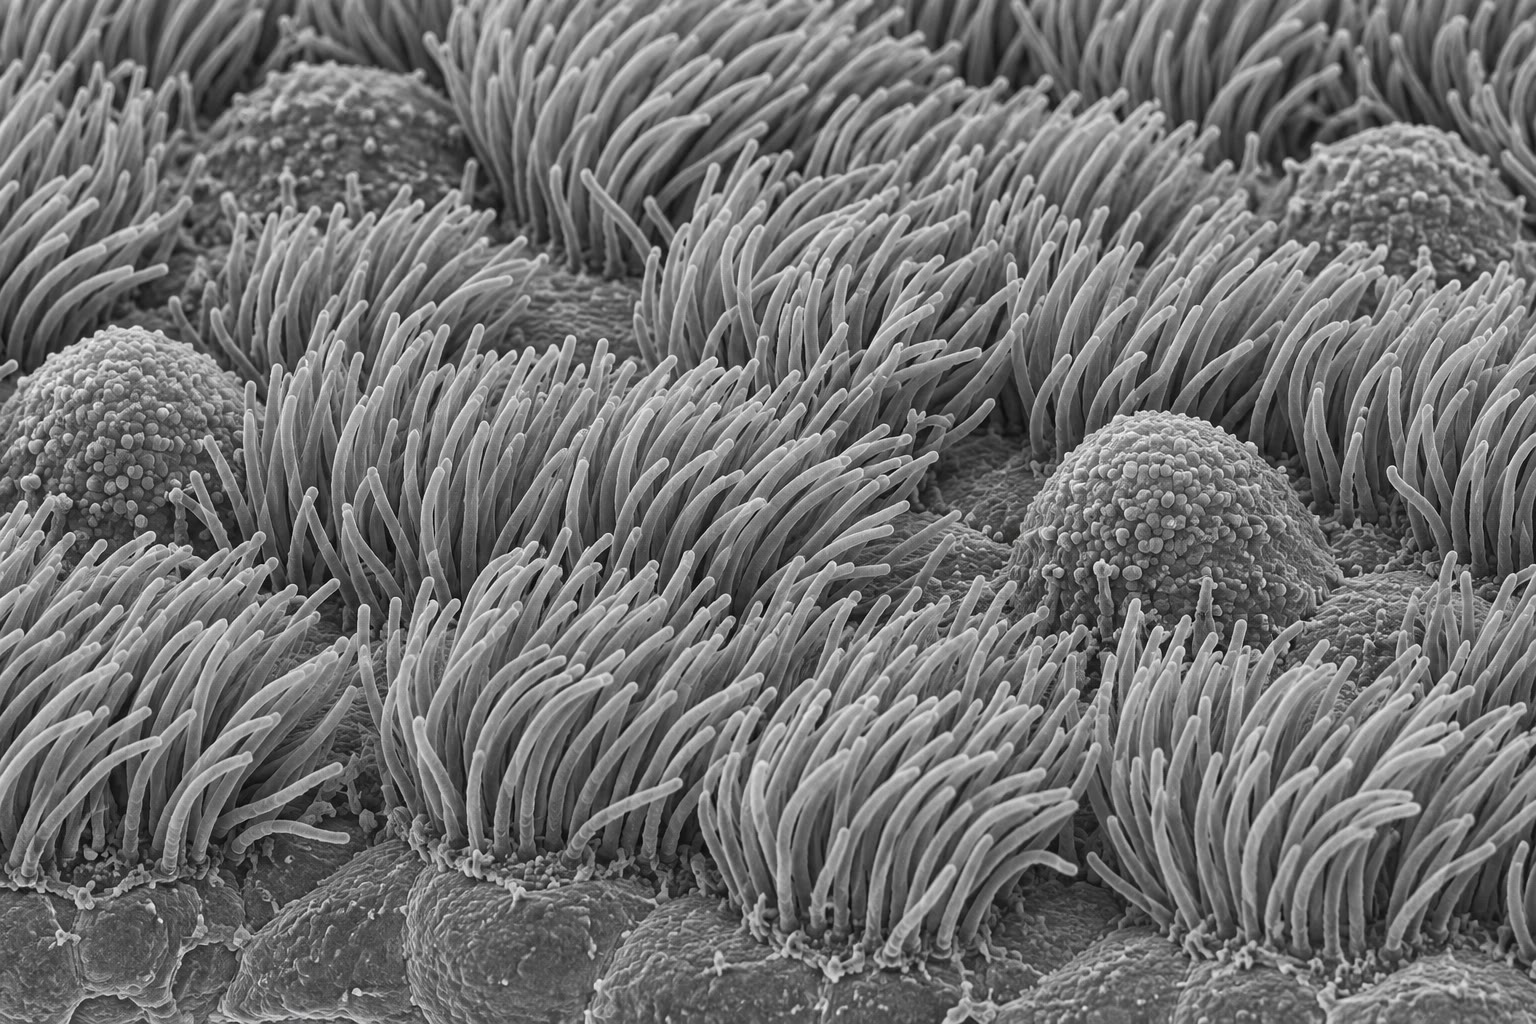
\includegraphics[width=0.54\linewidth]{images/book5/ai/b5-09-cilia-sem.jpg}\hspace{0.03\linewidth}
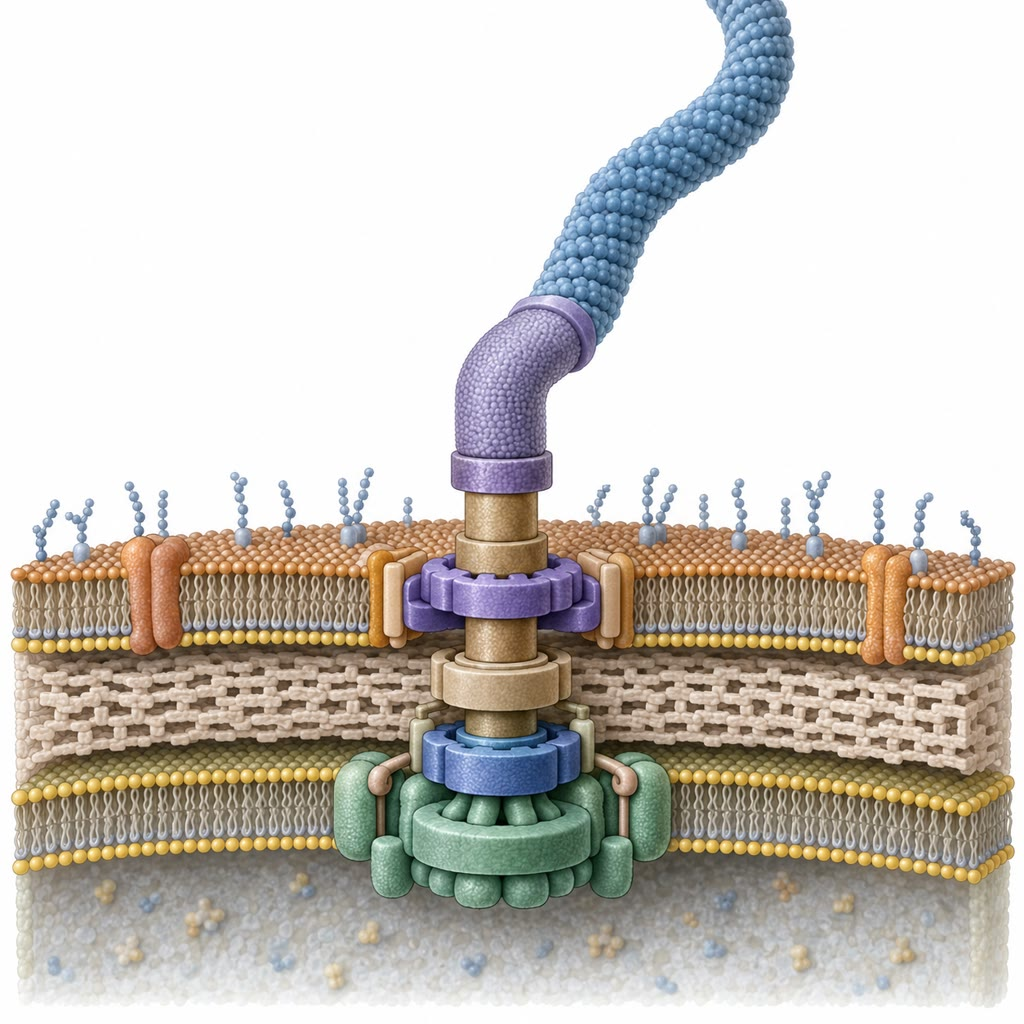
\includegraphics[width=0.36\linewidth]{images/book5/ai/b5-09-flagellar-motor.jpg}

{\small Left: the ciliated epithelium of the trachea in the scanning
electron microscope, a lawn of cilia among dome-shaped mucus-secreting
cells. Right: the bacterial \omterm{prop:b3:cytoskeleton-motility:flagellar-motor}{flagellar motor}, a rotary engine of rings
in the cell envelope driven by the flow of protons.}
\end{omfigure}

\begin{proposition}[The bacterial flagellar motor]\label{prop:b3:cytoskeleton-motility:flagellar-motor}
\index{flagellar motor}\index{run and tumble}
The bacterial flagellum is unrelated to the eukaryotic one: a rigid
helical filament of flagellin, \qty{20}{nm} thick and several
micrometres long, turned by a \emph{rotary motor} embedded in the cell
envelope --- a rotor of some forty-five proteins surrounded by a ring
of stator units, each a channel through which protons flow down their
gradient into the cell, about a thousand protons per revolution. The
motor spins at up to \qty{300}{Hz}, reverses direction in a
millisecond, and develops a torque of some \qty{1000}{pN.nm}; it is
built from about twenty proteins whose genes are switched on in the
order the parts are assembled, from the inside out. In \emph{E.~coli},
counterclockwise rotation bundles the several flagella into a
propeller and the cell \emph{runs} straight; a switch to clockwise
flies the bundle apart and the cell \emph{tumbles} to a new random
direction. The chemotaxis pathway biases nothing but the frequency of
tumbles --- fewer when conditions improve --- and that suffices to
climb a gradient.
\end{proposition}

\begin{remark}[The cytoskeleton is a verb]\label{rem:b3:cytoskeleton-motility:verb}
Almost nothing described in this chapter is a structure in the sense
that a bone is: the \omterm{def:b3:cytoskeleton-motility:migration}{lamellipodium} is a wave of polymerisation, the
spindle of \cref{ch:b3:cell-cycle-apoptosis} a steady state of growing
and collapsing \omterm{def:b3:cytoskeleton-motility:filaments}{microtubules}, the \omterm{def:b3:cytoskeleton-motility:cilia}{cilium}'s beat a switching pattern of
motors. Turnover is not a cost the cell tolerates but the mechanism
itself, which is why every one of these systems runs on nucleotide
hydrolysis and stops within minutes of ATP depletion, and why the
poisons that freeze the polymers in either state --- taxol or
colchicine, phalloidin or cytochalasin --- are equally lethal.
\end{remark}

\section{Exercises}

\begin{exercise}[$\star$]\label{exo:b3:cytoskeleton-motility:1}
Compare \omterm{def:b3:cytoskeleton-motility:filaments}{actin filaments}, \omterm{def:b3:cytoskeleton-motility:filaments}{microtubules} and \omterm{def:b3:cytoskeleton-motility:filaments}{intermediate filaments} in
diameter, subunit, polarity, nucleotide and typical role.
\end{exercise}

\begin{exercise}[$\star$]\label{exo:b3:cytoskeleton-motility:2}
Define \omterm{thm:b3:cytoskeleton-motility:treadmilling}{critical concentration}. Why do the two ends of an \omterm{def:b3:cytoskeleton-motility:filaments}{actin
filament} have different \omterm{thm:b3:cytoskeleton-motility:treadmilling}{critical concentrations}, and what would happen
if they were equal?
\end{exercise}

\begin{exercise}[$\star$]\label{exo:b3:cytoskeleton-motility:3}
Name a motor for each: vesicle toward the cell periphery on
\omterm{def:b3:cytoskeleton-motility:filaments}{microtubules}; vesicle toward the centre; contraction of a stress
fibre; bending of a \omterm{def:b3:cytoskeleton-motility:cilia}{cilium}. Give the direction each takes on its track.
\end{exercise}

\begin{exercise}[$\star$]\label{exo:b3:cytoskeleton-motility:4}
List the four steps of the crawling cycle and the Rho-family GTPase
that governs each of the first three.
\end{exercise}

\begin{exercise}[$\star\star$]\label{exo:b3:cytoskeleton-motility:5}
A polymer's plus end has $k_{\text{on}} = \qty{5}{\micro M^{-1}.s^{-1}}$,
$k_{\text{off}} = \qty{1}{s^{-1}}$, its minus end $k_{\text{on}} =
\qty{1}{\micro M^{-1}.s^{-1}}$, $k_{\text{off}} = \qty{0.8}{s^{-1}}$.
Find the two \omterm{thm:b3:cytoskeleton-motility:treadmilling}{critical concentrations}, the steady-state concentration
and the treadmilling rate in subunits per second and, for
\qty{2.7}{nm} subunits, in nanometres per second.
\end{exercise}

\begin{exercise}[$\star\star$]\label{exo:b3:cytoskeleton-motility:6}
\omterm{def:b3:cytoskeleton-motility:motors}{Kinesin} walks at \qty{800}{nm/s} with \qty{8}{nm} steps, one ATP each.
How many ATP per second per motor? A neuron's axon is \qty{1}{m}: how
long is the trip, and how many ATP does one motor spend on it? Compare
with the diffusion time from \cref{prop:b3:cytoskeleton-motility:physics}.
\end{exercise}

\begin{exercise}[$\star\star$]\label{exo:b3:cytoskeleton-motility:7}
\omterm{def:b3:cytoskeleton-motility:motors}{Myosin} V steps \qty{36}{nm} per ATP. What is its maximal \omterm{prop:b3:cytoskeleton-motility:physics}{stall force},
and why is it lower than \omterm{def:b3:cytoskeleton-motility:motors}{kinesin}'s? Which motor is better suited to
carrying a large load, and which to moving fast?
\end{exercise}

\begin{exercise}[$\star\star$]\label{exo:b3:cytoskeleton-motility:8}
Predict the effect on a dividing cell, and on a crawling cell, of (a)
taxol, (b) colchicine, (c) cytochalasin, (d) a Rac inhibitor, and
explain each from the mechanism.
\end{exercise}

\begin{exercise}[$\star\star$]\label{exo:b3:cytoskeleton-motility:9}
In a FRAP experiment on a \omterm{def:b3:cytoskeleton-motility:migration}{lamellipodium}, fluorescence recovers with a
half-time of \qty{20}{s} to \qty{90}{\%} of its initial value. What are
the residence time of actin in the network and the immobile fraction?
The speckles flow backward at \qty{1.5}{\micro m/min} while the edge
advances at \qty{1}{\micro m/min}: at what rate is actin polymerising
at the edge?
\end{exercise}

\begin{exercise}[$\star\star\star$]\label{exo:b3:cytoskeleton-motility:10}
Explain \omterm{def:b3:cytoskeleton-motility:instability}{dynamic instability} in terms of the \omterm{def:b3:cytoskeleton-motility:instability}{GTP cap}, and show why a
\omterm{def:b3:cytoskeleton-motility:filaments}{microtubule} population held just above the \omterm{thm:b3:cytoskeleton-motility:treadmilling}{critical concentration}
becomes bimodal in length rather than uniform. What does the cell gain
from a behaviour that wastes GTP?
\end{exercise}

\begin{exercise}[$\star\star\star$]\label{exo:b3:cytoskeleton-motility:11}
A bacterium of \qty{2}{\micro m} swims at \qty{25}{\micro m/s}. In
water at this scale viscous drag dominates and the cell stops within a
nanometre when the motor stops. Explain why a reciprocal motion (an
oar) cannot propel it and a rotating helix can, and estimate the
number of protons the motor spends per second at \qty{100}{Hz}.
\end{exercise}

\begin{exercise}[$\star\star\star$]\label{exo:b3:cytoskeleton-motility:12}
Kartagener syndrome --- immotile cilia --- gives chronic bronchitis,
male infertility, and in half of patients a heart on the right side.
Explain each from the biology of the \omterm{def:b3:cytoskeleton-motility:cilia}{axoneme}, and say why the last
affects only half.
\end{exercise}

\section{Problem: A Neutrophil on the Move}

\begin{problem}[{Weekend problem --- a neutrophil's actin budget
counted, its treadmilling computed, a vesicle's journey down an axon
timed against diffusion, a motor's efficiency measured, and the
crawling front's polymerisation and ATP cost worked out, ending on the
treadmilling rate, the time to cross an axon and the ATP a
lamellipodium burns per second}]
\label{pb:b3:cytoskeleton-motility:1}
Data: a neutrophil of volume \qty{300}{\micro m^3} holds actin at
\qty{200}{\micro M}, half polymerised; a subunit adds \qty{2.7}{nm} to a
filament. Actin rate constants as in
\cref{ex:b3:cytoskeleton-motility:actin-numbers}. \omterm{def:b3:cytoskeleton-motility:motors}{Kinesin}: \qty{8}{nm}
steps, \qty{800}{nm/s}, \omterm{prop:b3:cytoskeleton-motility:physics}{stall force} \qty{6}{pN}; ATP hydrolysis
$\Delta G = \qty{50}{kJ/mol}$; $k_{B}T = \qty{4.1}{pN.nm}$; vesicle
diffusion coefficient \qty{1}{\micro m^2/s}; axon length \qty{1}{m}. The
\omterm{def:b3:cytoskeleton-motility:migration}{lamellipodium} is \qty{20}{\micro m} wide with $200$ filaments per
micrometre of edge, advancing at \qty{10}{\micro m/min}; the network
is disassembled \qty{3}{\micro m} behind the edge.

\medskip
\noindent\textbf{Part I --- The actin budget.}
\begin{enumerate}
  \item How many actin molecules does the cell contain, and how many
        are in filaments?
  \item What total filament length is that? If the average filament is
        \qty{0.25}{\micro m}, how many filaments?
  \item The free actin is \qty{100}{\micro M}, far above the \omterm{thm:b3:cytoskeleton-motility:treadmilling}{critical
        concentration} of the barbed end. Why do the filaments not
        simply grow until the monomer is exhausted? (Two proteins.)
  \item Treadmilling in vitro: compute $C_{\text{ss}}$ and $J$ from the
        rate constants, and the treadmilling speed in nanometres per
        second and micrometres per minute.
  \item In the cell the effective speed is \qty{1}{\micro m/min}. By
        what factor do the regulators accelerate the bare polymer?
  \item Each treadmilled subunit costs one ATP. If all $2\times 10^{5}$
        filaments treadmilled at the cellular speed, how many ATP per
        second, and what fraction is that of a cell's total turnover of
        about $10^{9}$ ATP per second?
\end{enumerate}

\medskip
\noindent\textbf{Part II --- A vesicle down the axon.}
\begin{enumerate}[resume]
  \item How long does a kinesin-driven vesicle take to travel the axon,
        and how many steps and ATP does the motor spend?
  \item How long would diffusion take over \qty{1}{m}? Over
        \qty{10}{\micro m}, the width of a cell body? What does the
        comparison say about where cells can afford to rely on
        diffusion?
  \item Compute the energy per ATP in joules and in units of $k_{B}T$.
  \item The maximal force of a motor with \qty{8}{nm} steps, and
        \omterm{def:b3:cytoskeleton-motility:motors}{kinesin}'s efficiency at stall.
  \item A vesicle of \qty{100}{nm} radius in cytoplasm of viscosity
        \qty{0.01}{Pa.s} (ten times water) moving at \qty{800}{nm/s}
        feels a drag $F = 6\pi\eta r v$. Compute it, and compare with the
        \omterm{prop:b3:cytoskeleton-motility:physics}{stall force}: how many motors are needed?
  \item A neuron's axon carries about $10^{4}$ vesicles at a time. What
        is the total ATP consumption of the transport, per second, and
        how does it compare with the neuron's firing costs of about
        $10^{9}$ ATP per second? What does this imply for a neuron in
        which mitochondria fail?
\end{enumerate}

\medskip
\noindent\textbf{Part III --- The front.}
\begin{enumerate}[resume]
  \item Convert the edge speed to nanometres per second, and compute the
        number of subunits per second each filament must add to keep
        up.
  \item How many filaments push the edge, and how many subunits per
        second does the whole edge consume?
  \item Each subunit added is one ATP hydrolysed and later recycled.
        ATP per second for protrusion; fraction of the cell's $10^{9}$
        per second.
  \item The network behind the edge is \qty{3}{\micro m} deep and
        disassembles there. What is the lifetime of a subunit in the
        network, and how many subunits are in the network at any time?
  \item The membrane resists protrusion with a force of about
        \qty{1}{pN} per filament. Compute the work done per subunit
        added ($F\times \qty{2.7}{nm}$) in $k_{B}T$ and say whether the
        Brownian ratchet --- a thermal fluctuation opening a gap of
        \qty{2.7}{nm} --- is plausible.
  \item Why does a Listeria comet tail need no motor, and how fast can
        it push if it recruits the same machinery?
\end{enumerate}

\medskip
\noindent\textbf{Part IV --- Direction.}
\begin{enumerate}[resume]
  \item The neutrophil senses a chemoattractant whose concentration
        rises by \qty{2}{\%} across its \qty{10}{\micro m} width. With
        \num{50000} receptors and $K_{d}$ equal to the mean
        concentration, how many more receptors are occupied on the
        front half than on the back half? (Occupancy $\theta = C/(C +
        K_{d})$; use half the receptors per side.)
  \item The random fluctuation in the number occupied on one side is
        about the square root of the number. Is the difference of
        question 19 detectable in a single instant? How does averaging
        over a few seconds help?
  \item Which GTPase must be activated at the front and which at the
        rear for the cell to turn toward the source? What would a cell
        with constitutively active Rac everywhere do?
  \item The cell reaches the bacterium in \qty{3}{min} from
        \qty{30}{\micro m} away. Check the speed against the data.
  \item A cell lacking Arp2/3 moves by blebbing --- pressure-driven
        bulges of membrane --- instead. Which step of the cycle has
        been replaced, and what does it say about the role of actin in
        the other steps?
  \item The whole crawling cycle takes minutes, yet the cell turns
        within seconds when the gradient shifts. Explain, using the
        lifetime of the network from question~16.
  \item Summarise: the treadmilling speed in vitro (question~4), the
        time for a vesicle to travel the axon (question~7), and the ATP
        per second spent on protrusion (question~15).
\end{enumerate}
\end{problem}
